\documentclass[a4paper, 11pt]{article}
\usepackage{comment} % enables the use of multi-line comments (\ifx \fi) 
\usepackage{fullpage} % changes the margin
\usepackage{enumitem}
\usepackage[T1]{fontenc}
\usepackage[polish]{babel}
\usepackage[utf8]{inputenc}
\usepackage{ragged2e}
\usepackage{graphicx}
\usepackage{datatool}
\usepackage{rotating}
\usepackage{placeins}
\usepackage{pdflscape}
\usepackage{float}
\usepackage{listings}
\usepackage{pdfpages}
\usepackage{xcolor} % for setting colors
\usepackage{verbatim}
\usepackage{listings}

\usepackage{color}

\usepackage{tikz}

\usepackage{hyperref}
\hypersetup{
colorlinks,
citecolor=black,
filecolor=black,
linkcolor=black,
urlcolor=black
}

\lstdefinestyle{Java}{
language=Java,
basicstyle=\fontsize{11}{13}\selectfont\ttfamily,
numbers=left,
stepnumber=1,
numbersep=9pt,
tabsize=4,
frame = single,
showspaces=false,
showstringspaces=false
}

\lstdefinelanguage{JavaScript}{
keywords={typeof, new, true, false, catch, function, return, null, catch, switch, var, if, in, while, do, else, case, break},
keywordstyle=\color{blue}\bfseries,
ndkeywords={class, export, boolean, throw, implements, import, this},
ndkeywordstyle=\color{darkgray}\bfseries,
identifierstyle=\color{black},
sensitive=false,
comment=[l]{//},
morecomment=[s]{/*}{*/},
commentstyle=\color{purple}\ttfamily,
stringstyle=\color{red}\ttfamily,
morestring=[b]',
morestring=[b]"
}

\lstset{
language=JavaScript,
backgroundcolor=\color{white},
extendedchars=true,
basicstyle=\fontsize{11}{13}\selectfont\ttfamily,
showstringspaces=false,
showspaces=false,
numbers=left,
numberstyle=\footnotesize,
numbersep=9pt,
frame = single,
tabsize=2,
breaklines=true,
showtabs=false,
captionpos=b
}


\definecolor{dkgreen}{rgb}{0,0.6,0}
\definecolor{gray}{rgb}{0.5,0.5,0.5}
\definecolor{mauve}{rgb}{0.58,0,0.82}

\renewcommand{\thesubsection}{\thesection.\alph{subsection}}


\title{Raport z wykonania ćwiczenia MongoDB}
\author{Jakub Płotnikowski}
\date{Grudzień 2019r.}


\begin{document}

    \maketitle
    \tableofcontents

    \newpage

    \section{Wykorzystując bazę danych yelp dataset wykonaj zapytanie i komendy MongoDB,
    aby uzyskać następujące rezultaty:}


    \subsection{Zwróć bez powtórzeń wszystkie nazwy miast w których znajdują się firmy
    (business). }


    \lstinputlisting{source_code/task1/1a.js}

    \begin{center}
        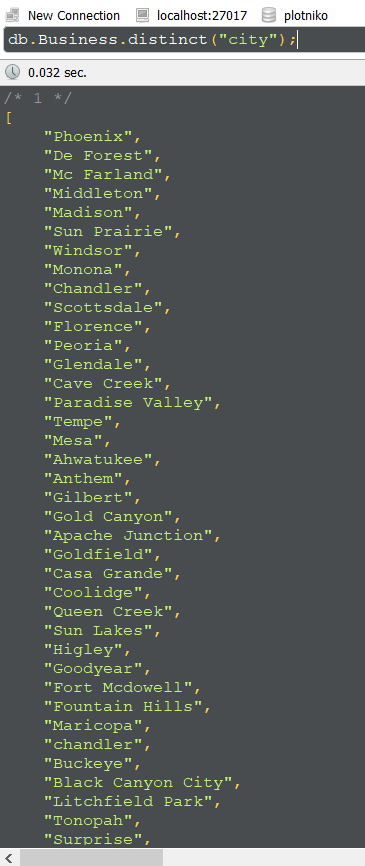
\includegraphics{images/task1/1a.png}
    \end{center}

    \newpage

    \subsection{Zwróć liczbę wszystkich recenzji, które pojawiły się w roku 2011 i 2012.}

    \lstinputlisting{source_code/task1/1b.js}

    \begin{center}
        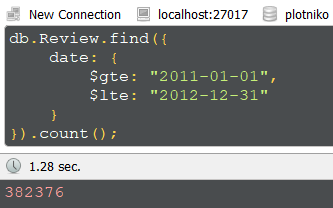
\includegraphics{images/task1/1b.png}
    \end{center}

    \newpage

    \subsection{Zwróć dane wszystkich otwartych (open) firm (business) z pól: id, nazwa, adres.}

    \lstinputlisting{source_code/task1/1c.js}

    \begin{center}
        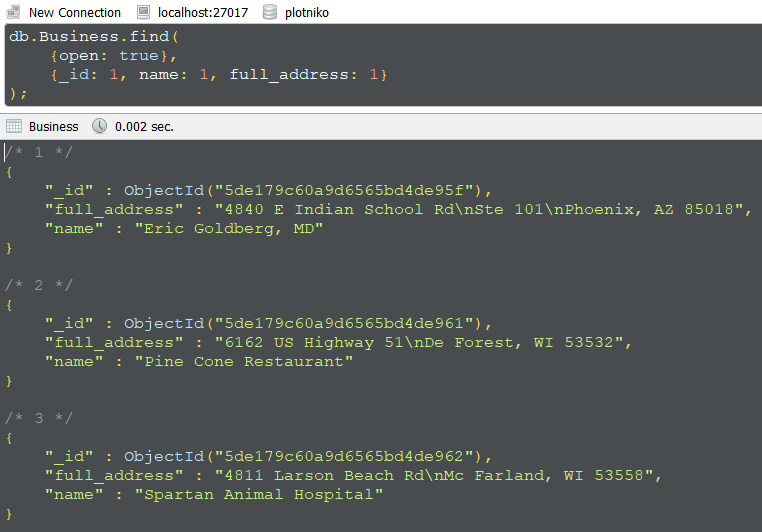
\includegraphics{images/task1/1c.png}
    \end{center}

    \newpage

    \subsection{Zwróć dane wszystkich użytkowników (user), którzy uzyskali przynajmniej jeden
    pozytywny głos z jednej z kategorii (funny, useful, cool), wynik posortuj
    alfabetycznie na podstawie imienia użytkownika.}

    \lstinputlisting{source_code/task1/1d.js}


    \begin{center}
        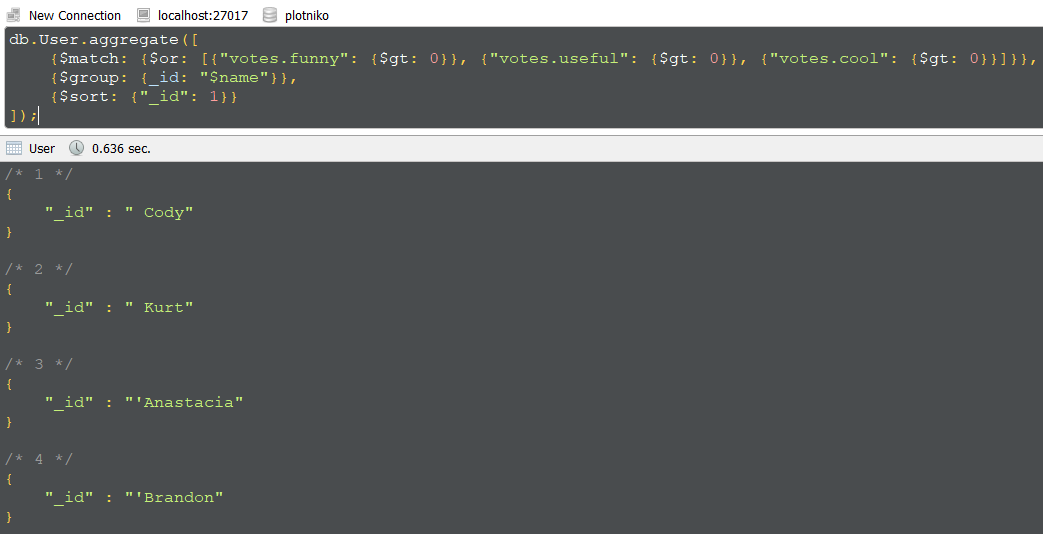
\includegraphics[scale=0.8]{images/task1/1d.png}
    \end{center}

    \newpage


    \subsection{Określ, ile każde przedsiębiorstwo otrzymało wskazówek/napiwków (tip) w 2013.
    Wynik posortuj alfabetycznie na podstawie nazwy firmy.}

    \lstinputlisting{source_code/task1/1e.js}

    \begin{center}
        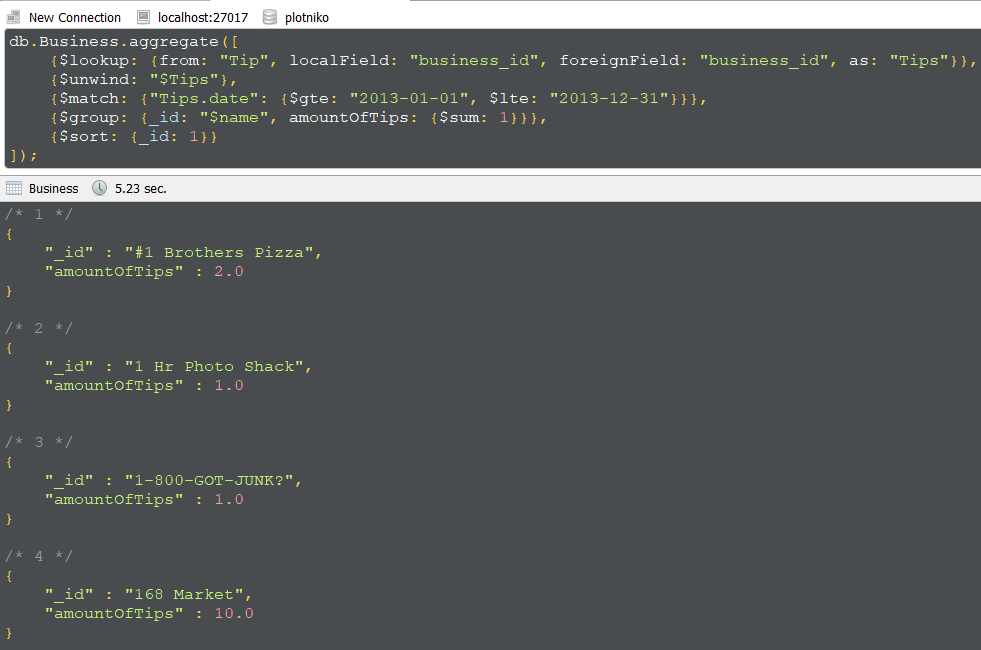
\includegraphics[scale=0.8]{images/task1/1e.png}
    \end{center}

    \newpage

    \subsection{Wyznacz, jaką średnia ocen (stars) uzyskała każda firma (business) na podstawie
    wszystkich recenzji, wynik posortuj on najwyższego uzyskanego wyniku. }

    \lstinputlisting{source_code/task1/1f.js}

    \begin{center}
        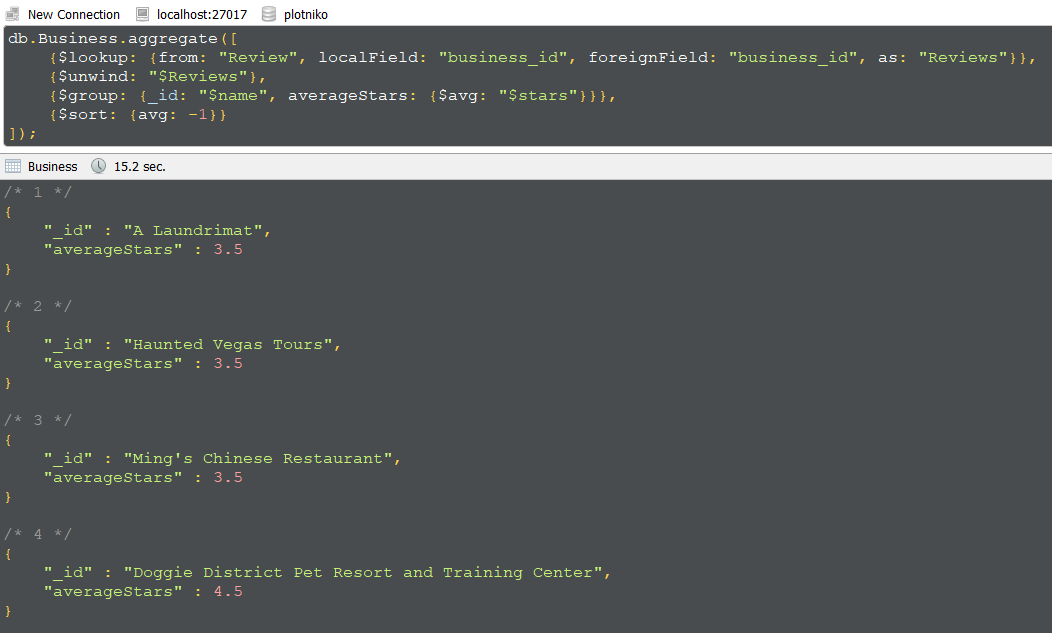
\includegraphics[scale=0.8]{images/task1/1f.png}
    \end{center}

    \newpage

    \subsection{Usuń wszystkie firmy (business), które posiadają ocenę (stars) poniżej 3. }

    \lstinputlisting{source_code/task1/1g.js}


    \newpage

    \section{Zdefiniuj funkcję (MongoDB) umożliwiającą dodanie nowej wskazówki/napiwku (tip).
    Wykonaj przykładowe wywołanie. }

    \lstinputlisting{source_code/task2/2.js}

    \begin{center}
        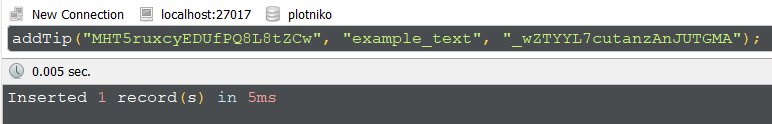
\includegraphics[scale=0.8]{images/task2/Execution.png}
    \end{center}

    \newpage


    \section{Zdefiniuj funkcję (MongoDB), która zwróci wszystkie wskazówki/napiwki (tip), w
    których w tekście znajdzie się fraza podana jako argument. Wykonaj przykładowe
    wywołanie zdefiniowanej funkcji. }

    \lstinputlisting{source_code/task3/3.js}

    \begin{center}
        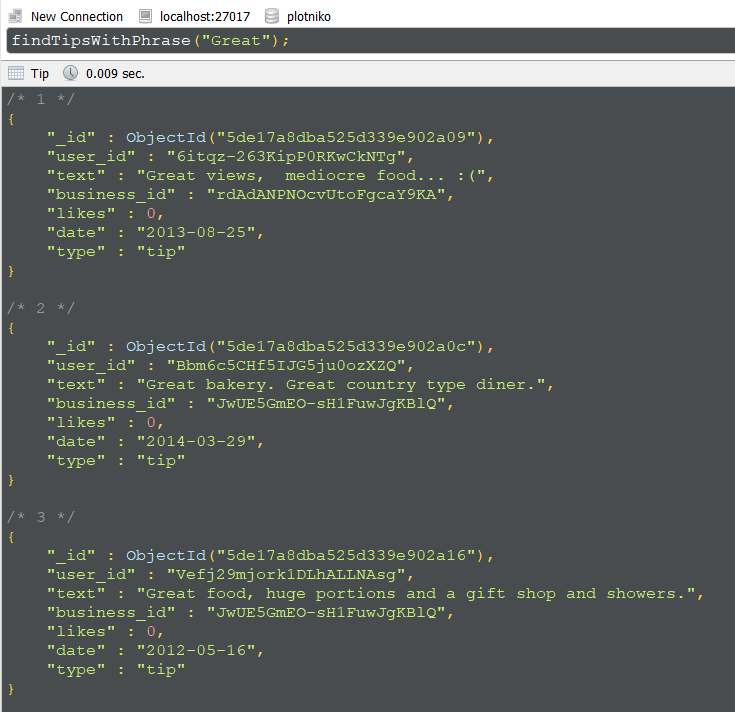
\includegraphics[scale=0.8]{images/task3/Execution.png}
    \end{center}

    \newpage

    \section{Zdefiniuj funkcję (MongoDB), która umożliwi modyfikację nazwy firmy (business) na
    podstawie id. Id oraz nazwa mają być przekazywane jako parametry. }

    \lstinputlisting{source_code/task4/4.js}

    \begin{center}
        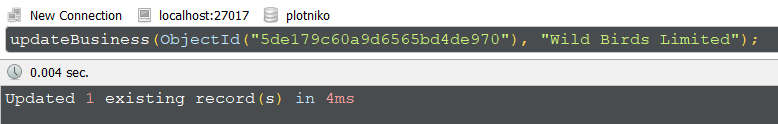
\includegraphics[scale=0.8]{images/task4/Execution.png}
    \end{center}

    \newpage

    \section{Zwróć średnia ilość wszystkich recenzji użytkowników, wykorzystaj map reduce}

    \lstinputlisting{source_code/task5/5.js}


    \newpage

    \section{Odwzoruj wszystkie zadania z punktu 1 w języku programowania (np. JAVA) z pomocą
    API do MongoDB. Wykorzystaj dla każdego zadania odrębną metodę. }

    \subsection{Zwróć bez powtórzeń wszystkie nazwy miast w których znajdują się firmy
    (business). }

    \lstinputlisting[style=Java,firstline=2,lastline=8]{source_code/task6/1a.java}

    \subsection{Zwróć liczbę wszystkich recenzji, które pojawiły się w roku 2011 i 2012}

    \lstinputlisting[style=Java,firstline=2,lastline=10]{source_code/task6/1b.java}


    \subsection{Zwróć dane wszystkich otwartych (open) firm (business) z pól: id, nazwa, adres.}

    \lstinputlisting[style=Java,firstline=2,lastline=10]{source_code/task6/1c.java}

    \newpage

    \subsection{Zwróć dane wszystkich użytkowników (user), którzy uzyskali przynajmniej jeden
    pozytywny głos z jednej z kategorii (funny, useful, cool), wynik posortuj
    alfabetycznie na podstawie imienia użytkownika.}


    \lstinputlisting[style=Java,firstline=2,lastline=19]{source_code/task6/1d.java}

    \subsection{Określ, ile każde przedsiębiorstwo otrzymało wskazówek/napiwków (tip) w 2013.
    Wynik posortuj alfabetycznie na podstawie nazwy firmy. }

    \lstinputlisting[style=Java,firstline=2,lastline=18]{source_code/task6/1e.java}

    \newpage

    \subsection{Wyznacz, jaką średnia ocen (stars) uzyskała każda firma (business) na podstawie
    wszystkich recenzji, wynik posortuj on najwyższego uzyskanego wyniku. }

    \lstinputlisting[style=Java,firstline=2,lastline=14]{source_code/task6/1f.java}


    \subsection{Usuń wszystkie firmy (business), które posiadają ocenę (stars) poniżej 3. }

    \lstinputlisting[style=Java,firstline=2,lastline=17]{source_code/task6/1g.java}

    \newpage

    \subsection{Cały kod klasy MongoDB}

    \lstinputlisting[style=Java,firstline=2,lastline=123]{source_code/main/MongoDB.java}

    \newpage


    \section{Zaproponuj bazę danych składającą się z 3 kolekcji pozwalającą przechowywać dane
    dotyczące: studentów, przedmiotów oraz sal zajęciowych. W bazie wykorzystaj: pola
    proste, złożone i tablice. Zaprezentuj strukturę dokumentów w formie JSON dla
    przykładowych danych. }

    \subsection{Kolekcja Students}

    \lstinputlisting{source_code/task7/createStudents.js}

    \lstinputlisting{source_code/task7/insertStudents.js}

    Przykład pobrania danych z kolekcji Students:

    \begin{center}
        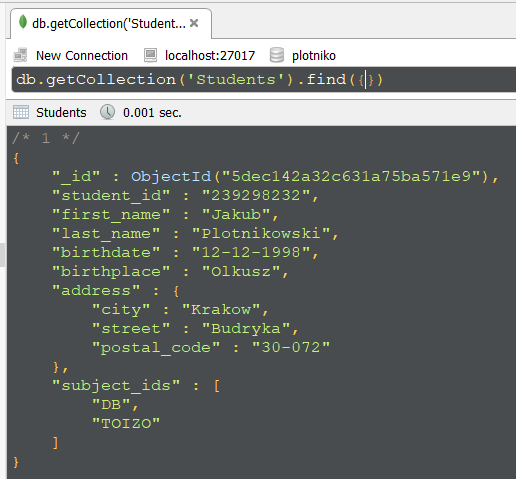
\includegraphics[scale=0.8]{images/task7/Students.png}
    \end{center}

    \newpage

    \subsection{Kolekcja Subjects}

    \lstinputlisting{source_code/task7/createSubjects.js}

    \lstinputlisting{source_code/task7/insertSubjects.js}

    Przykład pobrania danych z kolekcji Subjects:

    \begin{center}
        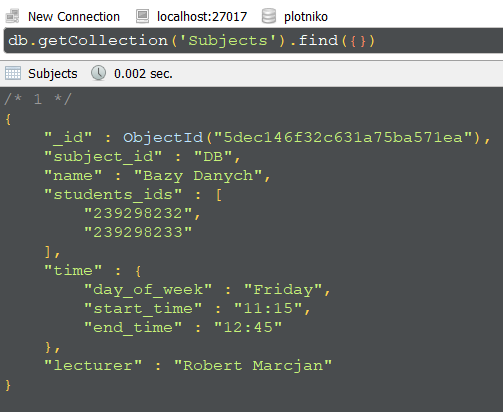
\includegraphics[scale=0.8]{images/task7/Subjects.png}
    \end{center}

    \newpage

    \subsection{Kolekcja Classes}

    \lstinputlisting{source_code/task7/createClasses.js}

    \lstinputlisting{source_code/task7/insertClasses.js}

    Przykład pobrania danych z kolekcji Classes:

    \begin{center}
        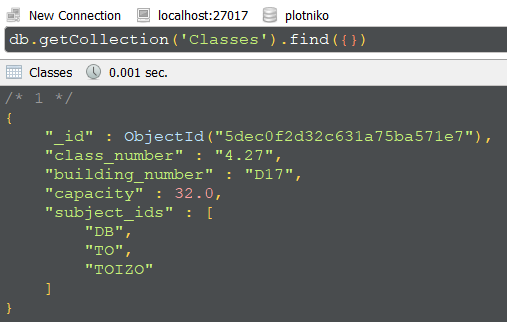
\includegraphics[scale=0.8]{images/task7/Classes.png}
    \end{center}


\end{document}